%% statlm_paper_vi.tex
%% Bài báo theo định dạng IEEE Conference (IEEEtran) -- bản tiếng Việt
%% Nội dung: StatLM - Phân loại văn bản đa nhãn tiếng Việt zero-shot
%%
%% HƯỚNG DẪN BIÊN DỊCH (khớp với toolchain của template IEEE conference đi kèm):
%%   pdflatex statlm_paper_vi
%%   bibtex   statlm_paper_vi
%%   pdflatex statlm_paper_vi
%%   pdflatex statlm_paper_vi
%% Yêu cầu: IEEEtran.cls, IEEEtran.bst và gói vntex (cung cấp "vietnam"/babel
%% tiếng Việt). Nếu môi trường không có vntex, có thể chuyển sang XeLaTeX và thay
%% khối font tiếng Việt bằng fontspec.

\documentclass[conference]{IEEEtran}
\IEEEoverridecommandlockouts
% Dòng trên chỉ cần khi khai báo nguồn tài trợ ở footnote đầu tiên. Nếu không có,
% có thể comment lại.

% ---- Tiếng Việt (pdflatex + vntex) ----
\usepackage[utf8]{inputenc}
\usepackage[T5]{fontenc}
\usepackage[utf8]{vietnam}

% ---- Toán, bảng, hình, trích dẫn ----
\usepackage{cite}
\usepackage{amsmath,amssymb,amsfonts}
\usepackage{algorithmic}
\usepackage{graphicx}
\usepackage{textcomp}
\usepackage{xcolor}
\usepackage{booktabs}
\usepackage{array}
\usepackage{multirow}
\usepackage{tabularx}
\usepackage{url}
\def\BibTeX{{\rm B\kern-.05em{\sc i\kern-.025em b}\kern-.08em
    T\kern-.1667em\lower.7ex\hbox{E}\kern-.125emX}}

\interdisplaylinepenalty=2500
\hyphenation{em-bed-ding key-phrase}

\begin{document}

\title{StatLM: Pipeline Lai cho Phân loại Văn bản\\
Đa nhãn Tiếng Việt theo hướng Zero-shot}

\author{\IEEEauthorblockN{1\textsuperscript{st} Nguyễn Quang Tuấn}
\IEEEauthorblockA{\textit{Trường Đại học Công nghệ} \\
\textit{Đại học Quốc gia Hà Nội} \\
Hà Nội, Việt Nam \\
nqtuan.code@gmail.com}
\and
\IEEEauthorblockN{2\textsuperscript{nd} Lê Khánh Trình}
\IEEEauthorblockA{\textit{Trường Đại học Công nghệ} \\
\textit{Đại học Quốc gia Hà Nội} \\
Hà Nội, Việt Nam \\
trinhlk@vnu.edu.vn}
}

\maketitle

\begin{abstract}
Trong bối cảnh bùng nổ dữ liệu số, nhu cầu tự động tổ chức và phân loại văn bản
ngày càng cấp thiết. Đây là một bài toán khó -- không gian nhãn và danh mục của
mỗi văn bản phải được khám phá mà không cần dữ liệu gán nhãn theo tác vụ -- và
các phương pháp hiện tại vẫn phải đánh đổi giữa chất lượng nhãn, chi phí gọi mô
hình ngôn ngữ lớn (LLM) và tốc độ xử lý. Bài báo đề xuất \textbf{StatLM}, một
kiến trúc lai (hybrid) kết hợp encoder thống kê và decoder mô hình ngôn ngữ lớn,
hướng tới phân loại văn bản đa nhãn zero-shot trong môi trường thế giới mở. Phần encoder dùng tóm tắt trích xuất TextRank
(trên nền sentence embedding tiếng Việt) để giảm nhiễu, sau đó dùng KeyBERT với
mô hình embedding bất đối xứng để cô đặc thông tin thành cụm từ khóa; phần
decoder chỉ huy động LLM đúng một lần ở khâu cuối để đặt tên và chuẩn hóa không
gian nhãn. Thực nghiệm trên bộ dữ liệu báo chí VietnamNet (2.000 bài, 20 chuyên
mục) cho thấy so với baseline X-MLClass-Gemini (cài đặt X-MLClass dùng LLM toàn
phần với backbone Gemini 2.5 Flash), StatLM nâng tỉ lệ nhãn thô (coarse) từ 32,6\% lên 76,9\%, hạ tỉ lệ nhãn
nhiễu từ 39,1\% xuống 3,8\%, và phủ 19/20 chuyên mục (so với 15/20). Về hiệu
năng, StatLM giảm thời gian xử lý trung bình từ 40 xuống 10 giây/bài, tiêu thụ
token LLM ít hơn khoảng 30 lần và chỉ gọi API một lần thay vì tám lần. Kết quả
khẳng định triết lý ``làm sạch trước, khái quát sau'' là một giải pháp hiệu quả,
cân bằng và phù hợp cho điều kiện tài nguyên hạn chế.
\end{abstract}

\begin{IEEEkeywords}
Encoder thống kê, gán nhãn thô (coarse labeling), KeyBERT, mô hình ngôn ngữ lớn,
phân loại văn bản đa nhãn zero-shot, pipeline lai (hybrid), StatLM, TextRank, xử
lý ngôn ngữ tự nhiên tiếng Việt.
\end{IEEEkeywords}

% ============================================================
\section{Giới thiệu}
% ============================================================
Sự bùng nổ của dữ liệu văn bản số tại Việt Nam -- từ báo điện
tử, thương mại điện tử, mạng xã hội đến kho lưu trữ học thuật -- khiến việc tổ
chức và phân loại thủ công ngày càng bất khả thi, đặt ra yêu cầu về các hệ thống
tự động hóa. Trong số đó, \emph{phân loại văn bản đa
nhãn zero-shot} (zero-shot multi-label text classification) trong môi trường thế
giới mở nổi lên như một bài toán then chốt: hệ thống tự động xác định không gian
nhãn (label space) và gán nhiều danh mục cho mỗi văn bản mà không cần bất kỳ dữ
liệu gán nhãn theo tác vụ hay tập nhãn định trước nào~\cite{li2024open}. Ở đây,
``thế giới mở'' (open-world) chỉ một môi trường động, nơi không gian nhãn không
được định trước mà được khám phá và mở rộng dần khi các batch dữ liệu mới đến
theo thời gian.

Một tình huống thực tế điển hình đến từ các công cụ quản lý tri thức cá nhân như
NotebookLM: người dùng tải lên hàng loạt tài liệu nhưng thiếu cơ chế tự động
phân cụm và phân cấp, buộc phải quản lý thủ công bằng thư mục hoặc đánh dấu chọn,
gây bất tiện khi số lượng tài liệu lớn.

Các hướng tiếp cận hiện có cho bài toán
này có thể chia thành ba nhóm~\cite{li2024open}. \emph{Thứ nhất}, học có giám sát
truyền thống cho độ chính xác cao nhưng cần tập nhãn đầy đủ và dữ liệu gán nhãn
-- trái với giả định không nhãn. \emph{Thứ hai}, dùng LLM để sinh nhãn trực tiếp
trên văn bản thô: linh hoạt nhưng chi phí gọi API rất lớn và dễ sinh nhãn nhiễu
do hạn chế cửa sổ ngữ cảnh. \emph{Thứ ba}, các phương pháp thống kê (mô hình chủ
đề, trích xuất từ khóa): nhanh, nhẹ, chi phí thấp nhưng chỉ trả về từ/cụm từ rời
rạc, thiếu tính khái quát để làm tên nhãn.

Từ đó nổi lên một khoảng trống rõ rệt: cần một giải pháp dung hòa được
\emph{chất lượng}, \emph{chi phí} và \emph{tốc độ}, đặc biệt cho tiếng Việt --
ngôn ngữ đơn lập, giàu từ đồng nghĩa và chưa được tối ưu tốt bởi các mô hình đa
ngữ. Bài báo này đề xuất \textbf{StatLM} (\emph{Statistical Encoder -- Language
Model Decoder}), một kiến trúc pipeline tách biệt vai trò giữa thành phần thống
kê và LLM. Ý tưởng cốt lõi: một \emph{encoder thống kê} đảm nhiệm giảm nhiễu và
cô đặc thông tin cốt lõi từ văn bản thô, trong khi \emph{decoder LLM} chỉ được
huy động tập trung một lần ở khâu đặt tên nhãn cuối cùng. Sự phân tách này cho
phép StatLM tận dụng đồng thời tốc độ của kỹ thuật thống kê và sức mạnh khái quát
hóa ngữ nghĩa của LLM.

Bài báo đặt ra ba câu hỏi nghiên cứu. \textbf{RQ1:} Những hạn chế nào tồn tại
trong các phương pháp phân loại đa nhãn zero-shot hiện nay, và kiến trúc
encoder--decoder khắc phục chúng ra sao? \textbf{RQ2:} Việc thay hàm tương đồng
từ vựng của TextRank bằng sentence embedding và tùy chỉnh KeyBERT cho tiếng Việt
cải thiện chất lượng tóm tắt và trích xuất keyphrase đến mức nào? \textbf{RQ3:}
Với việc chỉ dùng LLM ở decoder, StatLM cân bằng giữa chất lượng không gian nhãn,
chi phí và tốc độ ra sao so với hướng dùng LLM toàn phần?

\textbf{Đóng góp.} (i) Hệ thống hóa hạn chế của ba nhóm phương pháp và định vị
khoảng trống nghiên cứu, từ đó đề xuất kiến trúc encoder--decoder. (ii) Thiết kế
và triển khai pipeline StatLM hoàn chỉnh cho tiếng Việt, trong đó từng tầng được
lựa chọn công nghệ một cách có nguyên lý (thay hàm tương đồng của TextRank, cấu
hình KeyBERT bất đối xứng). (iii) Xây dựng và công bố công khai bộ dữ liệu
VietnamNet, cùng đánh giá thực nghiệm định lượng và định tính chứng minh hiệu quả
của giải pháp.



% ============================================================
\section{Nền tảng và Nghiên cứu liên quan}
\label{sec:related}
% ============================================================

\subsection{Tóm tắt văn bản trích xuất dựa trên đồ thị}
Tóm tắt văn bản tự động rút gọn văn bản gốc nhưng vẫn bảo toàn thông tin cốt
lõi. So với tóm tắt tóm lược (abstractive), tóm tắt trích
xuất (extractive) có ưu thế về tốc độ, tính trung thực và không cần dữ liệu huấn
luyện -- những yếu tố then chốt trong bối cảnh không giám sát và tránh ``ảo
giác'' (hallucination). Trong họ
trích xuất, hướng dựa trên đồ thị mô hình hóa văn bản thành mạng lưới câu và đánh
giá tầm quan trọng dựa trên cấu trúc toàn cục, không cần huấn luyện. TextRank áp
dụng PageRank vào miền văn bản và được
dùng rộng rãi~\cite{mihalcea2004textrank}, nhưng chất lượng phụ thuộc vào hàm đo
độ tương đồng. Phiên bản gốc dùng Word Overlap chỉ phản ánh tương đồng bề mặt từ
vựng; nhiều cải tiến đã được đề xuất (TF-IDF, LexRank, BM25+, và TextRank mở
rộng kết hợp LDA với hệ số giảm chấn điều chỉnh động~\cite{vora2024extractive}) song
vẫn giới hạn ở đặc trưng từ vựng.
Các nghiên cứu khuyến nghị chuyển sang sentence embedding để nắm bắt ngữ nghĩa
sâu hơn~\cite{kadriu2021extractive}.

\subsection{Trích xuất cụm từ khóa}
Các phương pháp trích xuất keyphrase không giám sát chia thành ba
nhóm. Nhóm \emph{thống kê} (TF-IDF, RAKE~\cite{rose2010automatic},
YAKE~\cite{campos2020yake}) nhanh nhẹ nhưng không
nắm bắt ngữ nghĩa. Nhóm \emph{đồ thị} (TextRank~\cite{mihalcea2004textrank},
TopicRank~\cite{bougouin2013topicrank}, Multipartite~\cite{boudin2018unsupervised},
WordAttractionRank~\cite{wang2014corpus}) cải thiện hơn nhưng thiếu cơ chế giảm
trùng lặp ở mức ngữ nghĩa. Nhóm \emph{embedding} đưa cả văn bản và ứng viên vào
cùng không gian vector: KeyBERT~\cite{grootendorst2020keybert} chọn các n-gram có
độ tương đồng cosine cao nhất với văn bản và có thể tích hợp Maximal Marginal
Relevance (MMR)~\cite{carbonell1998use} để tăng đa dạng. Một điểm mấu chốt là
\emph{tính bất đối xứng} của bài toán KeyBERT: một bên là tài liệu dài, một bên
là keyphrase rất ngắn; nếu mô hình embedding không được huấn luyện cho quan hệ
``truy vấn ngắn -- tài liệu dài'', chất lượng sẽ không tối ưu.

\subsection{Khám phá không gian nhãn}
Mô hình hóa chủ đề trải qua ba thế hệ: (i) dựa trên ``túi từ'' như LDA, NMF;
(ii) dựa trên embedding và phân cụm như Top2Vec, BERTopic; (iii) dùng LLM để
sinh và đặt tên chủ đề như TopicGPT. Hạn chế chung là thiên về gán
\emph{một} chủ đề cho mỗi văn bản, khó mở rộng sang kịch bản đa nhãn. Gần đây,
X-MLClass~\cite{li2024open} khai thác LLM một cách có hệ thống để khám phá không
gian nhãn đa nhãn (chia chunk, sinh keyphrase, phân cụm, lặp khám phá nhãn hiếm),
đạt độ phủ vượt trội so với các phương pháp truyền thống trên nhiều benchmark
tiếng Anh. Tuy nhiên, X-MLClass đòi hỏi LLM xử lý toàn bộ văn bản thô, dẫn đến
chi phí token lớn, tốc độ chậm, và trên dữ liệu báo chí giàu thực thể dễ sinh
nhãn nhiễu (entity, meta). StatLM kế thừa ý tưởng cốt lõi của X-MLClass nhưng đặt
một encoder thống kê phía trước để lọc nhiễu và chỉ cho LLM làm việc với keyphrase
đã được cô đặc.

\subsection{Tài nguyên xử lý tiếng Việt}
StatLM sử dụng hai công cụ tách từ tùy theo nhu cầu: \emph{pyvi}~\cite{pyvi} (nhẹ,
chỉ tách từ) và \emph{VnCoreNLP}~\cite{vu2018vncorenlp} (đồng thời tách từ, gán
nhãn từ loại và nhận dạng thực thể). Hai mô hình embedding chuyên biệt được dùng:
\emph{dangvantuan/vietnamese-embedding}~\cite{dangvantuan2021vietnamese} -- một
Sentence-BERT~\cite{reimers2019sentence} trên nền PhoBERT~\cite{nguyen2020phobert}
tối ưu cho tương đồng ngữ nghĩa đối xứng (STS, Pearson 84,21 trên
vi-stsbenchmark); và
\emph{bkai-foundation-models/vietnamese-bi-encoder}~\cite{nguyen2025improving} --
một Bi-Encoder huấn luyện cho truy xuất bất đối
xứng, đứng đầu benchmark VCS tiếng Việt.



% ============================================================
\section{Phương pháp StatLM}
% ============================================================
StatLM được thiết kế theo kiến trúc encoder--decoder ba tầng (Hình~\ref{fig:arch}).
Mỗi văn bản thô lần lượt đi qua hai tầng encoder thống kê (tóm tắt, trích xuất
keyphrase); tập keyphrase của tất cả văn bản sau đó được chuyển tới tầng decoder,
nơi LLM thực hiện phân cụm, đặt tên và gán nhãn. Đầu ra là một không gian nhãn
(các chủ đề có tên tiếng Việt) cùng danh sách nhãn cho mỗi văn bản. Pipeline hỗ
trợ xử lý tăng dần (incremental), bảo đảm tính thế giới mở (open-world).

Mặc dù pipeline có sử dụng các mô hình giám sát không phụ thuộc tác vụ
(task-agnostic) như bộ gán nhãn từ loại và các embedding tiền huấn luyện cho xử
lý ngôn ngữ nền tảng, tác vụ cốt lõi -- khám phá không gian nhãn và phân loại --
được thực hiện hoàn toàn theo hướng zero-shot, không dùng dữ liệu huấn luyện
theo miền.

\begin{figure*}[!t]
\centering
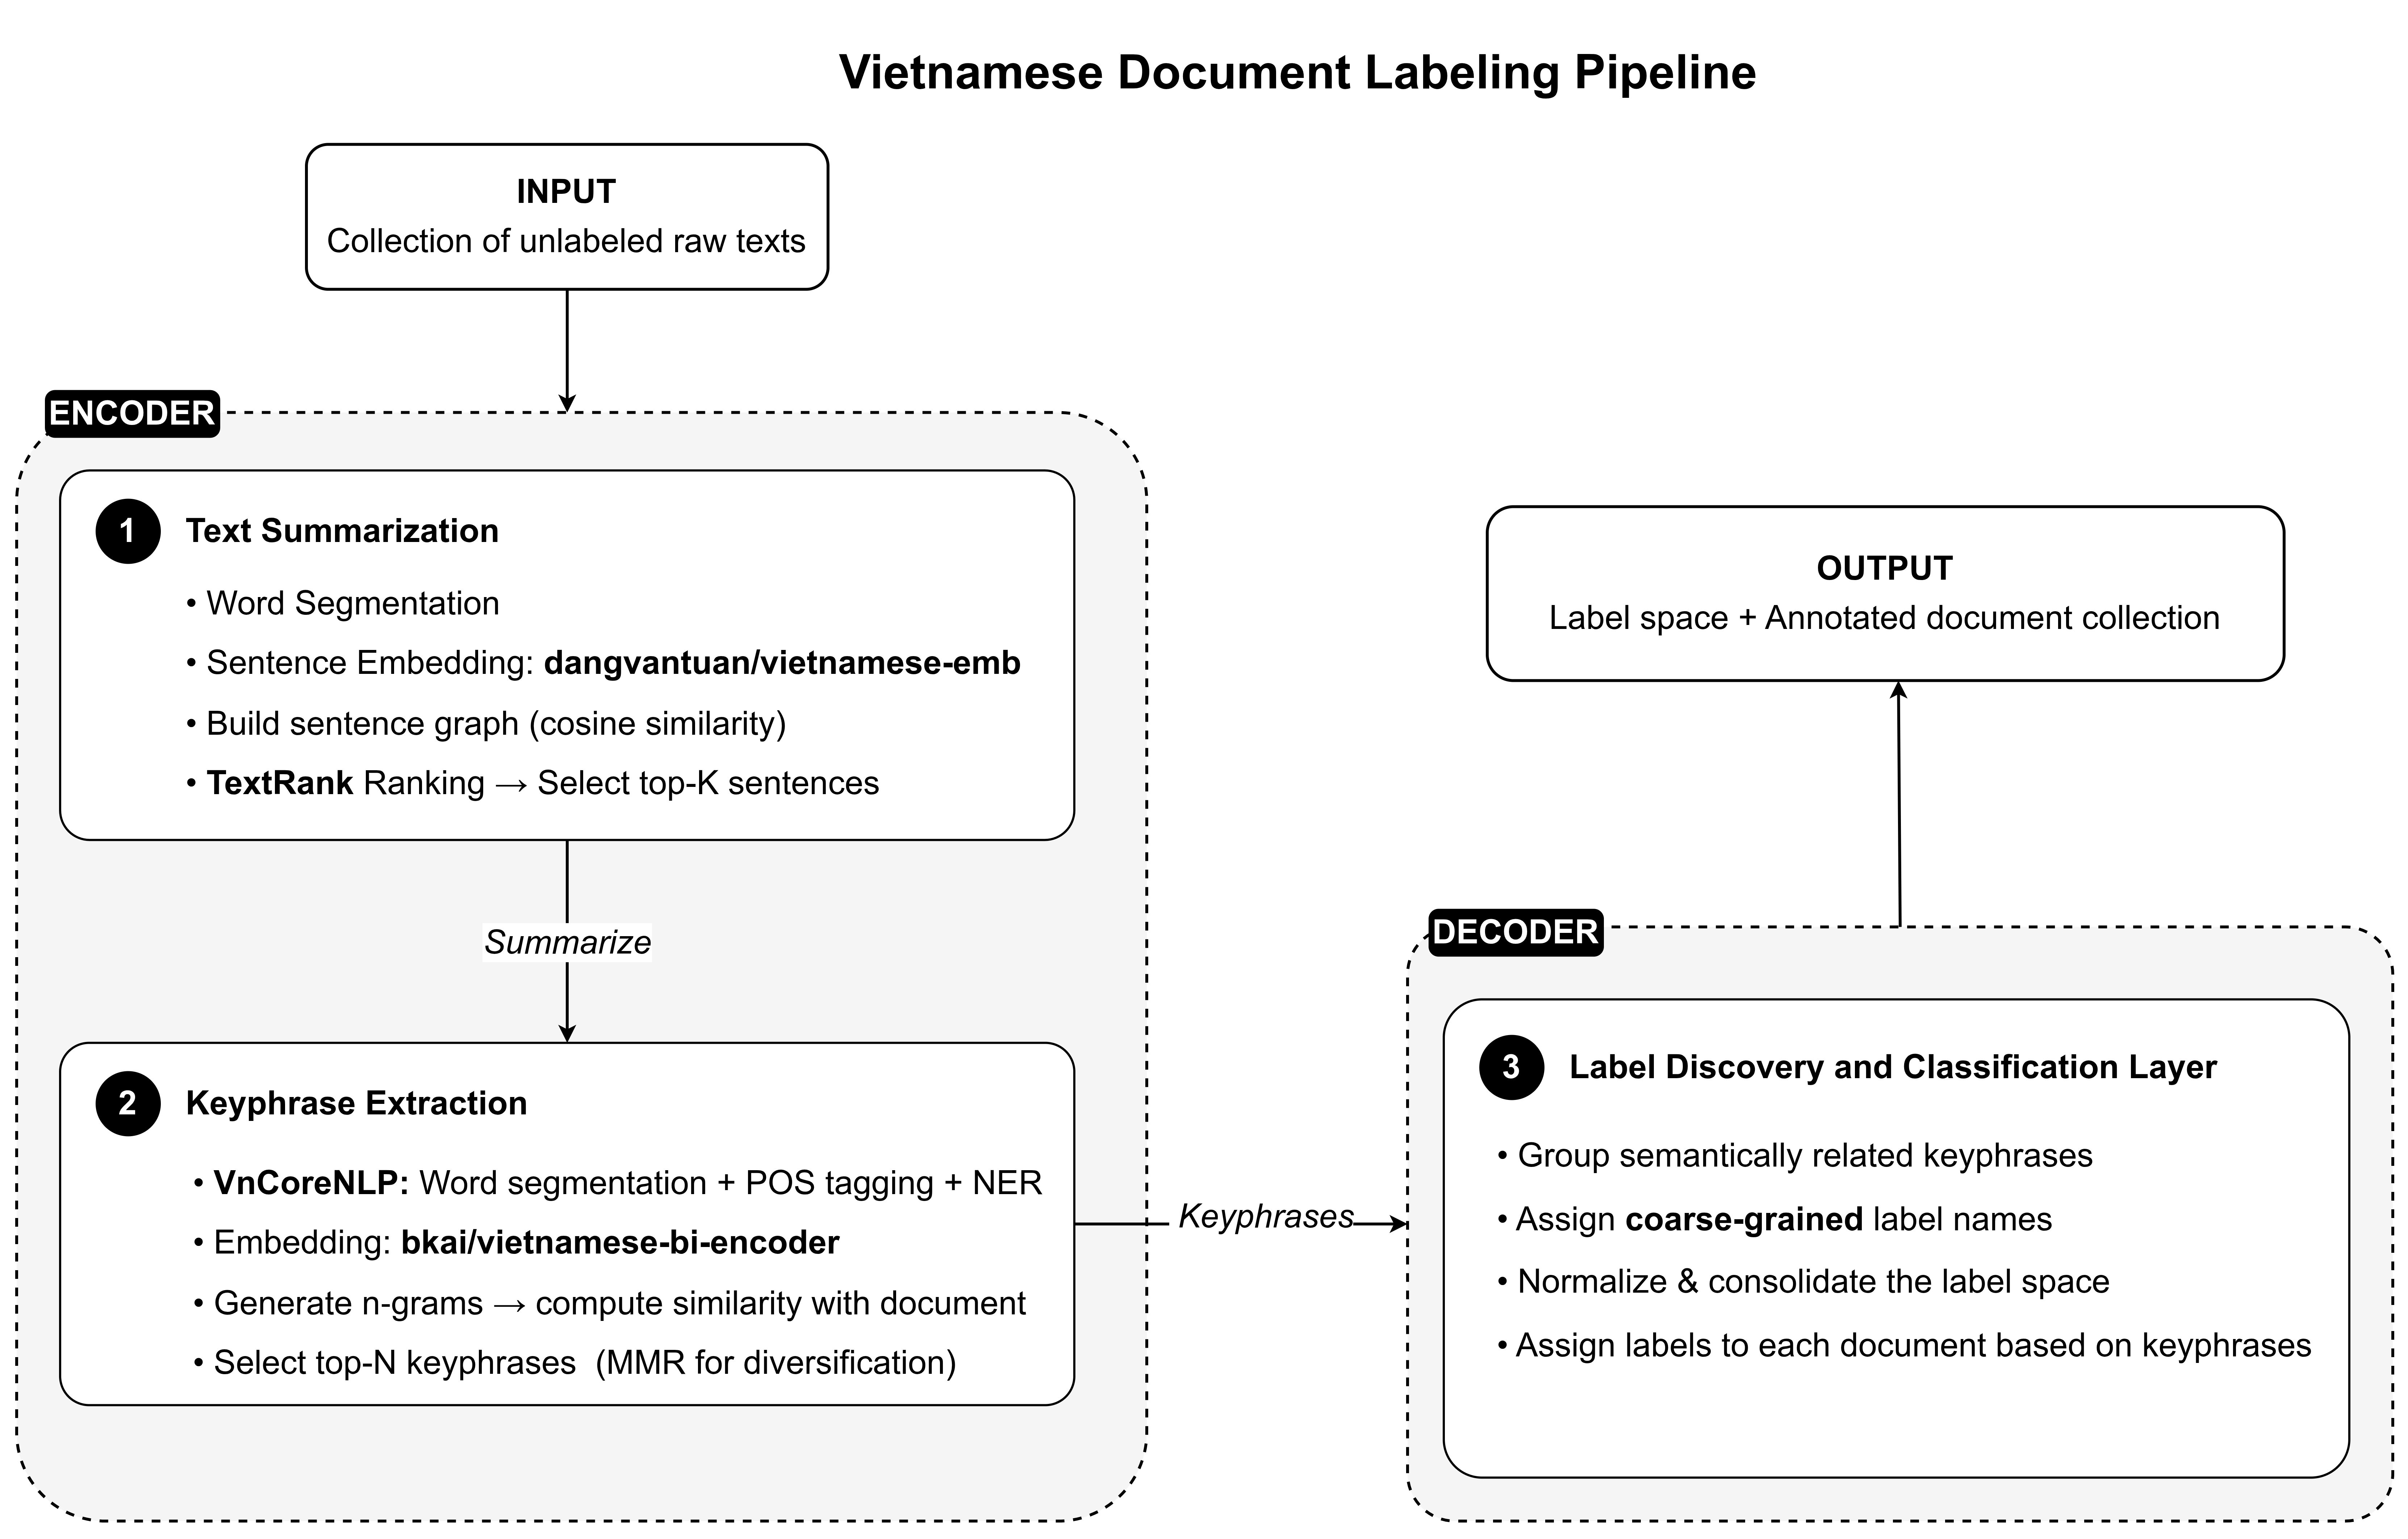
\includegraphics[width=0.95\textwidth]{figures/overview.png}
\caption{Kiến trúc tổng thể của StatLM: encoder thống kê gồm hai tầng (tóm tắt
văn bản với TextRank + \emph{dangvantuan/vietnamese-embedding}; trích xuất
keyphrase với KeyBERT + \emph{bkai/vietnamese-bi-encoder} và VnCoreNLP) làm nhiệm
vụ giảm nhiễu, cô đặc thông tin; decoder LLM (Gemini) chỉ được gọi một lần ở cuối
để khám phá, đặt tên và chuẩn hóa không gian nhãn rồi gán nhãn cho từng văn bản.}
\label{fig:arch}
\end{figure*}

\subsection{Tầng 1 -- Tóm tắt văn bản}
\textbf{Mục tiêu:} từ văn bản thô $D=\{s_1,\dots,s_n\}$ gồm $n$ câu, sinh bản tóm
tắt $S=\{s'_1,\dots,s'_k\}$ ($k<n$) nhằm loại bỏ câu ít quan trọng, tập trung vào
nội dung cốt lõi làm đầu vào cho Tầng~2.

Dựa trên phân tích ở Mục~\ref{sec:related}, StatLM chọn tóm tắt trích xuất dựa trên đồ thị câu
với thuật toán xếp hạng TextRank (PageRank cho hiệu suất tốt nhất và ổn định nhất
trong các độ đo trung tâm~\cite{kadriu2021extractive}). Điểm khác biệt then chốt
nằm ở \emph{hàm đo độ tương đồng}: thay vì Word Overlap, TF-IDF, BM25+ hay LDA
(đều chỉ phản ánh từ vựng bề mặt hoặc quá cồng kềnh), StatLM thực hiện bước nhảy
từ tương đồng từ vựng lên \emph{tương đồng ngữ nghĩa} bằng sentence embedding.
Bài toán ở đây có bản chất Semantic Textual Similarity \emph{đối xứng} (câu so
với câu, độ dài tương đương), nên StatLM dùng mô hình
\emph{dangvantuan/vietnamese-embedding}~\cite{dangvantuan2021vietnamese} cùng công
cụ tách từ pyvi để bảo đảm nhất quán giữa huấn luyện và suy luận.

Quy trình gồm năm bước: (1) tách câu bằng biểu thức chính quy, tách từ bằng pyvi;
(2) mã hóa mỗi câu thành vector $\mathbf{e}_i=\mathrm{meanpool}(\mathrm{PhoBERT}
(s_i))\in\mathbb{R}^{768}$; (3) xây đồ thị đầy đủ có trọng số với
$W_{ij}=\cos(\mathbf{e}_i,\mathbf{e}_j)$; (4) xếp hạng câu bằng TextRank với hệ số
giảm chấn $d=0{,}85$, ngưỡng hội tụ $\varepsilon=10^{-5}$ theo công thức cập nhật
\begin{equation}
\mathrm{WS}(v_i)^{(t+1)} = (1-d) + d\!\!\sum_{v_j\in \mathrm{In}(v_i)}
\frac{w_{ji}}{\sum_{v_k\in \mathrm{Out}(v_j)} w_{jk}}\,\mathrm{WS}(v_j)^{(t)};
\label{eq:textrank}
\end{equation}
(5) chọn $k$ câu điểm cao nhất ($k=\max(5,\lceil 0{,}4n\rceil)$ khi $n>5$) và sắp
xếp lại theo thứ tự gốc để bảo toàn mạch lạc. Hình~\ref{fig:textrank} minh họa đồ
thị câu đầy đủ có trọng số cùng bước xếp hạng của Tầng~1.

\begin{figure}[!t]
\centering
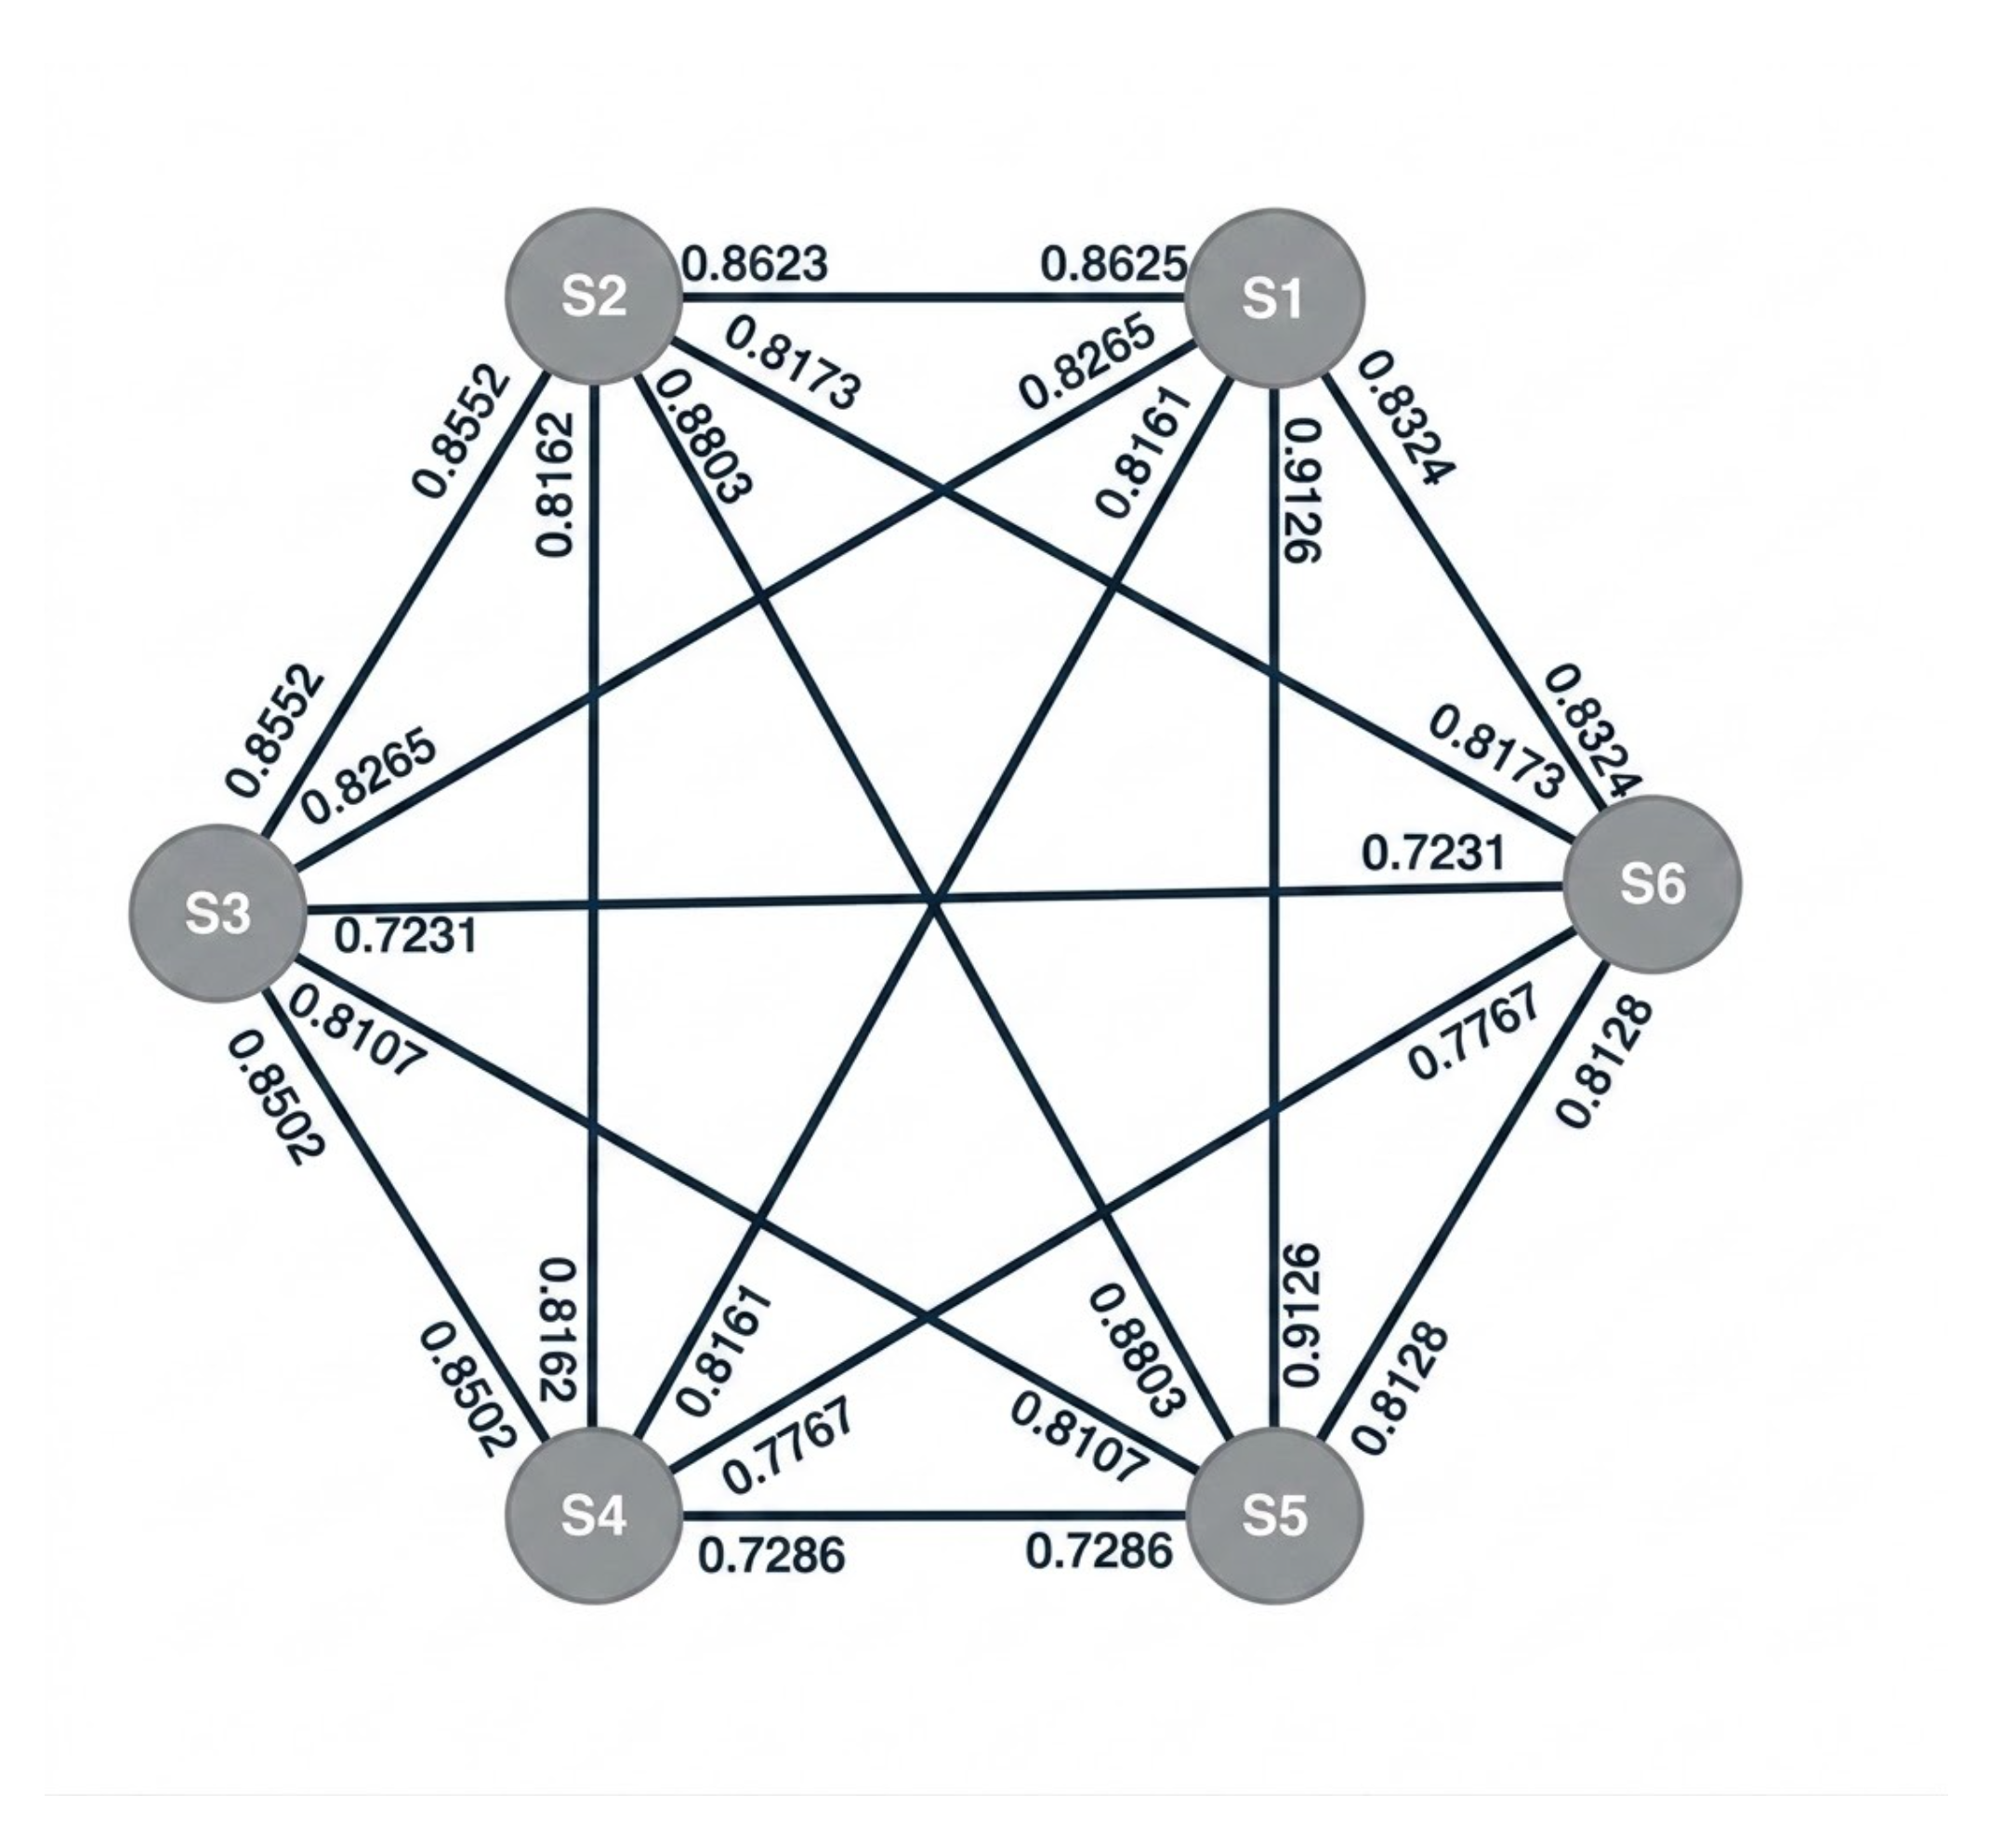
\includegraphics[width=0.92\columnwidth]{figures/stage1.png}
\caption{Đồ thị câu đầy đủ có trọng số ở Tầng~1: mỗi nút là một câu, trọng số
cạnh là độ tương đồng cosine giữa hai sentence embedding
(\emph{dangvantuan/vietnamese-embedding}); TextRank (PageRank) xếp hạng các nút và
chọn top-$k$ câu làm bản tóm tắt.}
\label{fig:textrank}
\end{figure}

\textbf{Về hệ số giảm chấn.} Chúng tôi cố định $d=0{,}85$ thay vì tinh chỉnh: đây
là giá trị kinh điển của PageRank~\cite{brin1998anatomy} và TextRank
gốc~\cite{mihalcea2004textrank}, và số hạng ``dịch chuyển'' $(1-d)$ trong
Eq.~\eqref{eq:textrank} chỉ để bảo đảm bước đi ngẫu nhiên ergodic, không mã hóa
thiên lệch theo ngữ liệu, nên \emph{thứ hạng} câu---và phép chọn top-$k$ mà Tầng~1
dùng---được ghi nhận là ổn định với $d$ trong dải chuẩn $[0{,}8;0{,}9]$. Chúng tôi
cũng tránh hướng ngược lại là hệ số giảm chấn \emph{động}: Extended TextRank của Vora
và cộng sự~\cite{vora2024extractive} kết hợp điểm LDA toàn cục và tính $d$ theo từng
tài liệu, nhưng chi phí LDA cùng trọng số kết hợp phải tinh chỉnh theo từng bộ dữ
liệu (ví dụ $0{,}1$ cho CNN/DailyMail so với $0{,}8$ cho BBC) đưa trở lại đúng kiểu
hiệu chỉnh bán giám sát mà StatLM muốn tránh. Việc cố định $d=0{,}85$ vì thế giữ
Tầng~1 không giám sát, để lại ngân sách giữ câu $r$ (bên dưới) là tham số Tầng~1 duy
nhất tương tác với dữ liệu.

\textbf{Về các câu bị bỏ.} Một câu bị \emph{loại bỏ} khi điểm TextRank
$\mathrm{WS}(s_i)$ trong Eq.~\eqref{eq:textrank} nằm ngoài nhóm top-$k$; do điểm này
tích lũy độ tương đồng ngữ nghĩa có trọng số giữa câu với toàn bộ văn bản, khoảng
$60\%$ câu bị loại là các nút có độ trung tâm thấp---câu diễn đạt lại dư thừa, câu
chuyển ý, câu khuôn mẫu và những câu lề liên kết yếu với lõi văn bản. Một chủ đề
chính được nhắc lại qua nhiều câu và gần như không bao giờ bị mất, trong khi một chủ
đề phụ chỉ hiện diện ở vài câu có độ trung tâm thấp có thể rơi dưới ngưỡng cắt và,
vì pipeline là vòng hở, không thể khôi phục ở các tầng sau. Tỉ lệ giữ lại được chọn
theo thực nghiệm: quét $r\in[0{,}2;0{,}6]$ (Bảng~\ref{tab:retention}) cho thấy độ gần
lõi tiêu đề+sapo giảm theo $r$ còn độ phủ chủ đề tăng, nên chúng tôi lấy mốc vận hành
$40\%$. Việc đặt ngân sách theo \emph{tỉ lệ} ($k=\max(5,\lceil 0{,}4n\rceil)$) thay vì
lead-$k$ cố định cho các chủ đề phụ nằm cuối bài cơ hội tồn tại, nhất quán với việc
TextRank trên embedding vượt Lead-$K$ về ROUGE (Bảng~\ref{tab:rouge}).

\subsection{Tầng 2 -- Trích xuất cụm từ khóa}
\textbf{Mục tiêu:} từ bản tóm tắt $S$, trích $m$ keyphrase (mặc định $m=10$, mỗi
cụm 1--3 từ) đại diện các khía cạnh nội dung chính, làm đầu vào cho Tầng~3.

StatLM dùng KeyBERT~\cite{grootendorst2020keybert}. Khác với Tầng~1, bài toán
KeyBERT mang bản chất \emph{bất đối xứng} (keyphrase ngắn so với tài liệu dài),
nên một mô hình xuất sắc cho STS đối xứng không đương nhiên tối ưu ở đây. StatLM
do đó chọn mô hình embedding riêng cho Tầng~2:
\emph{bkai-foundation-models/vietnamese-bi-encoder}~\cite{nguyen2025improving},
vốn được huấn luyện cho truy xuất ``truy vấn ngắn $\rightarrow$ tài liệu dài''
(Legal Text Retrieval) -- trùng khớp với cơ chế của KeyBERT. Tầng~2 còn dùng
VnCoreNLP~\cite{vu2018vncorenlp} để gán nhãn từ loại (chỉ giữ danh từ, danh từ
riêng, động từ, tính từ làm ứng viên n-gram) và nhận dạng thực thể (bảo toàn thực
thể có tên).

Quy trình: (1) tiền xử lý bằng VnCoreNLP, lọc stopword và lọc theo từ loại; (2)
mã hóa văn bản tóm tắt thành $\mathbf{E}_{doc}$; (3) sinh tập n-gram ứng viên
(1--3 từ) trong từng mảnh câu, bổ sung các thực thể NER; (4) tính độ tương đồng
\begin{equation}
\cos(\mathbf{E}_{doc},\mathbf{E}_{ngram}) =
\frac{\mathbf{E}_{doc}\cdot \mathbf{E}_{ngram}}
{\lVert \mathbf{E}_{doc}\rVert\,\lVert \mathbf{E}_{ngram}\rVert};
\label{eq:cosine}
\end{equation}
(5) chọn keyphrase bằng MMR~\cite{carbonell1998use} để cân bằng độ liên quan và
tính đa dạng:
\begin{equation}
\mathrm{MMR} = \arg\max_{c\notin S}\Big[\lambda\,\mathrm{sim}(c,doc)
-(1-\lambda)\max_{s\in S}\mathrm{sim}(c,s)\Big],
\label{eq:mmr}
\end{equation}
với $\lambda=0{,}5$ và ngưỡng trùng lặp tối đa $\theta=0{,}7$.

\textbf{Về các tham số MMR.} Chúng tôi đặt $\lambda$ ở trung điểm trung tính $0{,}5$,
điểm cân bằng giữa thuần liên quan ($\lambda\!\to\!1$) và thuần đa dạng
($\lambda\!\to\!0$)~\cite{carbonell1998use}: tập 5 keyphrase gửi xuống Tầng~3 phải
cùng nhau \emph{bao phủ} các khía cạnh của văn bản, nên thiên về liên quan sẽ lấp
danh sách bằng các biến thể gần trùng của cụm trung tâm nhất, còn thiên về đa dạng
lại nạp những cụm liên quan lỏng lẻo trở thành nhiễu nhãn. Ngưỡng trùng lặp
$\theta=0{,}7$ là phần bổ trợ ``cứng'' cho hình phạt ``mềm'' nói trên---một ứng viên
bị loại khi cosine với một keyphrase đã chọn vượt $\theta$---được đặt thận trọng để
các khía cạnh khác biệt nhưng gần chủ đề vẫn được giữ trong khi loại các cụm gần đồng
nghĩa hay trùng thành phần. Vì ứng viên đã được lọc từ loại và NER, hai số hạng nằm
trên cùng thang cosine và việc chọn ổn định quanh $(\lambda,\theta)=(0{,}5;0{,}7)$.

Quy trình của Tầng~2 được minh họa trong Hình~\ref{fig:keybert}. Như thể hiện trong hình, văn
bản tóm tắt và tập n-gram ứng viên (được bổ sung các thực thể có tên) được mã hóa
độc lập bởi \emph{bkai/vietnamese-bi-encoder}, và ma trận tương đồng cosine giữa
chúng quyết định việc xếp hạng. Sau đó, MMR vận hành trên ma trận này để chọn ra
top-$k$ keyphrase đa dạng, phản ánh bản chất bất đối xứng của bài toán so khớp
(tài liệu dài so với keyphrase ngắn). Bảng~\ref{tab:emb} đối chiếu
hai mô hình embedding được dùng ở hai tầng -- minh họa nguyên lý ``mỗi tầng dùng
đúng loại embedding phù hợp với bản chất bài toán''.

\begin{figure*}[!t]
\centering
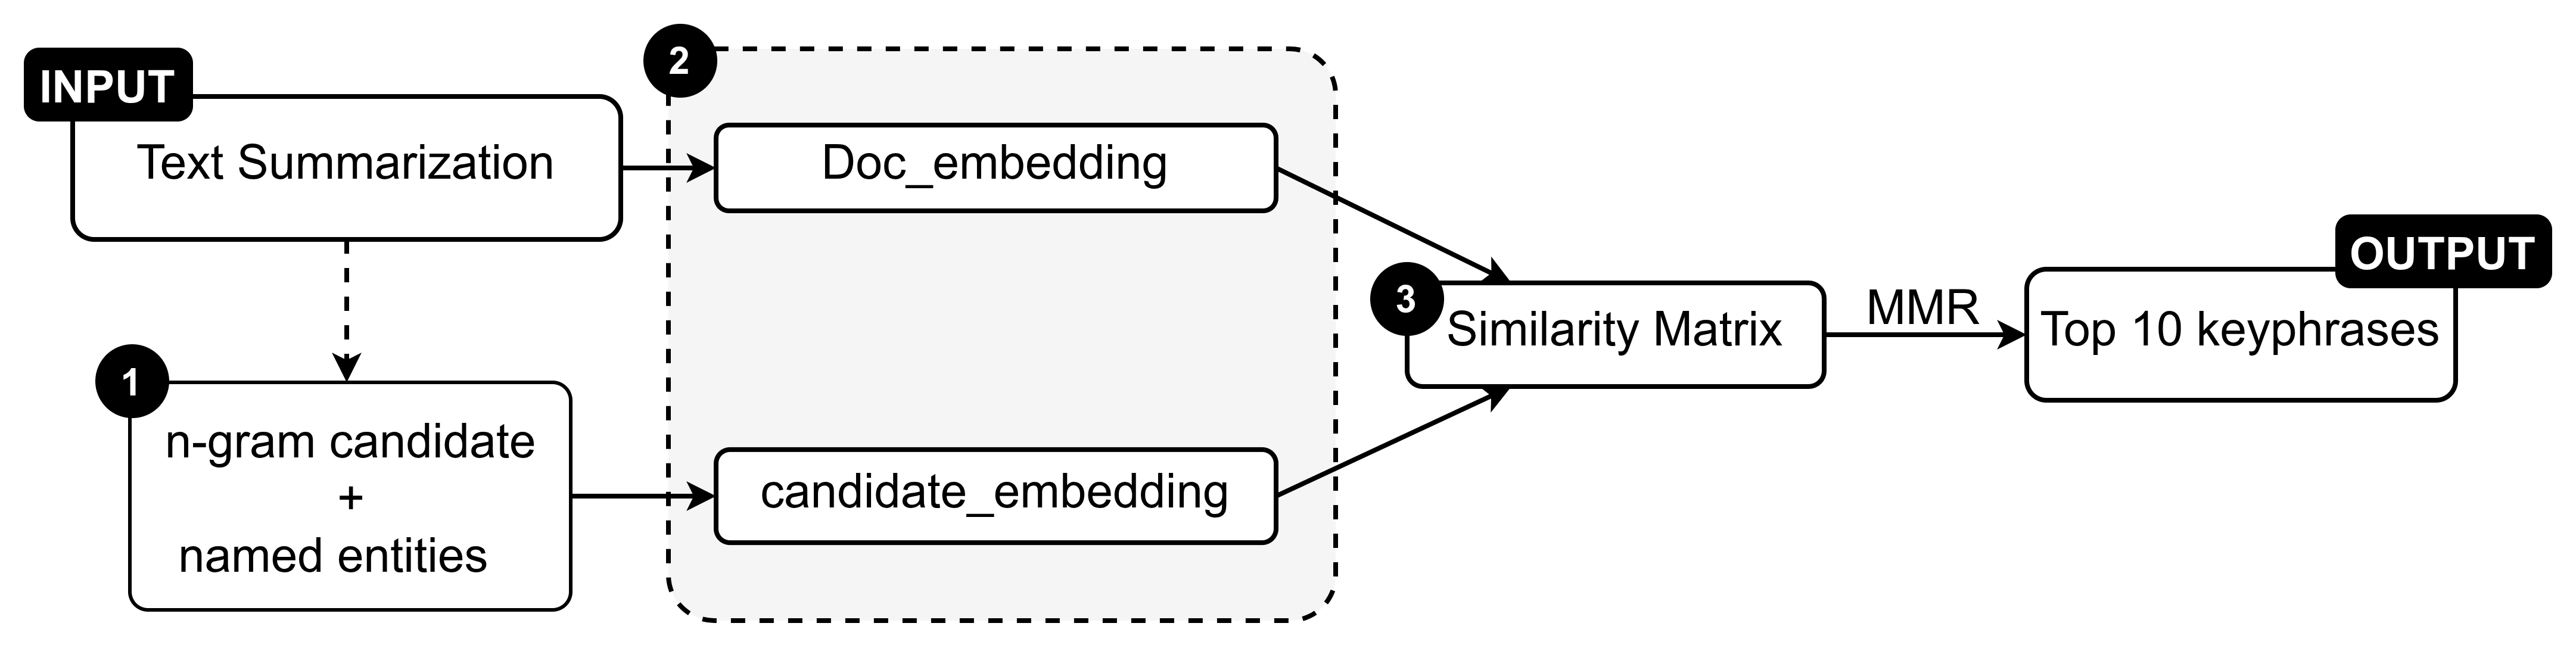
\includegraphics[width=0.95\textwidth]{figures/stage2.png}
\caption{Quy trình Tầng~2 (KeyBERT): văn bản tóm tắt và tập n-gram ứng viên (kèm
thực thể có tên) được mã hóa độc lập bằng \emph{bkai/vietnamese-bi-encoder}; ma
trận tương đồng cosine giữa chúng được dùng để xếp hạng, và MMR chọn ra top-$k$
keyphrase đa dạng. Đây là một bài toán bất đối xứng (tài liệu dài -- keyphrase
ngắn).}
\label{fig:keybert}
\end{figure*}

\begin{table}[!t]
\renewcommand{\arraystretch}{1.25}
\caption{Đối chiếu hai mô hình embedding trong StatLM}
\label{tab:emb}
\centering
\scriptsize
\begin{tabularx}{\columnwidth}{@{}lXX@{}}
\toprule
\textbf{Tiêu chí} & \textbf{Tầng 1 (TextRank)} & \textbf{Tầng 2 (KeyBERT)} \\
\midrule
Bài toán   & STS (đối xứng) & Truy xuất (bất đối xứng) \\
Quan hệ    & câu $\leftrightarrow$ câu & keyphrase ngắn $\leftrightarrow$ tài liệu dài \\
Mô hình    & dv-embedding & bkai-bi-encoder \\
Tách từ    & pyvi & VnCoreNLP \\
Đánh giá   & Pearson 84,21 & \#1 VCS retrieval \\
\bottomrule
\end{tabularx}
\end{table}

\subsection{Tầng 3 -- Phân loại và gán nhãn với LLM}
\textbf{Mục tiêu:} từ tập keyphrase $\mathcal{P}=\{p_1,\dots,p_N\}$ của $N$ văn
bản, tự động khám phá không gian nhãn $\mathcal{L}=\{l_1,\dots,l_M\}$ và gán nhãn
cho từng văn bản.

StatLM đặt LLM (Gemini 2.5 Flash) ở vị trí \emph{decoder} cuối pipeline, sau khi
dữ liệu đã được lọc và cô đặc. Cách thiết kế này giảm mạnh số token gửi đến API
(chỉ gửi keyphrase, không gửi văn bản thô) và hạn chế nhãn nhiễu (LLM không bị
phân tán bởi thực thể/định dạng trong văn bản gốc). Tầng~3 hoạt động theo ba bước, hỗ
trợ cả dữ liệu mới hoàn toàn lẫn dữ liệu bổ sung tăng dần: (1) với mỗi văn bản,
chỉ gửi tối đa 5 keyphrase điểm cao nhất để LLM chuẩn hóa; (2) gán văn bản vào các
cụm hiện có theo chiến lược ``nghiêm ngặt'', cho phép đề xuất đổi tên nhãn, đưa
văn bản không khớp vào danh sách ``chưa gán''; (3) phân cụm và đặt tên cho các văn
bản chưa gán. LLM được System Message hướng dẫn sinh nhãn ở mức khái quát
(coarse-grained), tránh nhãn quá chi tiết hay mang tính thực thể (ví dụ ``Giáo
dục'' thay vì ``Tuyển sinh đại học 2024''), đồng thời tối thiểu hóa số nhãn và
gộp các chủ đề tương đồng.



% ============================================================
\section{Thiết lập thực nghiệm}
% ============================================================
\textbf{Bộ dữ liệu.} Thực nghiệm tiến hành trên \emph{VietnamNet}, gồm 2.000 bài
báo phân bố đều trên 20 chuyên mục (100 bài/chuyên mục), mỗi bài 500--800 từ kèm
tiêu đề, sapo (đoạn dẫn nhập) và danh sách keyphrase. Đánh giá tóm tắt, trích xuất keyphrase và phân loại đều thực hiện trên toàn bộ
2.000 bài. Tùy tác vụ, các thành phần được
dùng làm tham chiếu: tiêu đề + sapo làm tóm tắt tham chiếu; danh sách keyphrase do
LLM (DeepSeek~V4) sinh làm tham chiếu keyphrase~\cite{pavlovic2024effectiveness};
và 20 chuyên mục gốc làm
\emph{coarse-label proxy} cho không gian nhãn (do không tồn tại ground-truth
tuyệt đối~\cite{wan2024tnt}).

\textbf{Môi trường \& tham số.} Toàn bộ thực nghiệm chạy trên máy cá nhân CPU
Intel Core i7 thế hệ 12, 16\,GB RAM, không GPU; các mô hình embedding chạy trên
CPU qua \texttt{sentence-transformers}; LLM truy cập qua Google API. Tham số cố
định: Tầng~1 ($d=0{,}85$, $\varepsilon=10^{-5}$, 40\% số câu, tối thiểu 5); Tầng~2
(n-gram $1$--$3$, $m=10$, MMR $\lambda=0{,}5$); Tầng~3 (\texttt{gemini-2.5-flash},
Temperature $0{,}1$ cho phân loại và $0{,}3$ cho sinh nhãn, gửi tối đa 5
keyphrase/bài).

\textbf{Baseline.} Đối với tóm tắt: Lead-K, TextRank gốc (Word Overlap), TextRank
+ TF-IDF. Đối với keyphrase: RAKE, YAKE, TextRank từ khóa, TopicRank, Multipartite,
WordAttractionRank, KeyBERT + embedding đối xứng. Đối với khám phá không gian nhãn
end-to-end: \emph{X-MLClass-Gemini} -- bản cài đặt của X-MLClass~\cite{li2024open} giữ nguyên
mô tả gốc (chunk 50 token, 4 keyphrase/chunk, BERTopic, NLI entailment, 10 vòng
lặp long-tail). Chúng tôi gọi baseline này là X-MLClass-Gemini vì nó tuân theo
pipeline X-MLClass và chỉ thay LLM gốc bằng Gemini 2.5 Flash để đồng nhất backbone
khi so sánh.

\textbf{Độ đo.} Tóm tắt dùng ROUGE-1/2/L (F1). Keyphrase dùng Precision/Recall/F1
tại $k=5,10$ với cơ chế so khớp kết hợp \emph{exact match} và \emph{soft match}
(cosine $\geq 0{,}7$). Không gian nhãn được phân tích định tính bằng cách xếp mỗi
nhãn vào một trong năm nhóm thủ công -- \emph{Coarse}, \emph{Long-tail}, \emph{Entity},
\emph{Meta/Noise}, \emph{Cross-topic} -- từ đó trích ba chỉ số: tỉ lệ Coarse, tỉ
lệ Nhiễu (Entity+Meta/Noise) và số chuyên mục được phủ. Chất lượng gán nhãn đầu
cuối dùng Precision-at-$k$:
\begin{equation}
P@k = \frac{1}{N}\sum_{i=1}^{N}
\frac{\lvert C_i^{rk}\cap L_i\rvert}{\min(k,\lvert L_i\rvert)},
\label{eq:pak}
\end{equation}
trong đó $C_i^{rk}$ là $k$ nhãn dự đoán hàng đầu và $L_i$ là tập nhãn tham chiếu.
Do thiếu nhãn đa nhãn ground-truth, chuyên mục gốc được dùng làm $L_i$ với
$\lvert L_i\rvert=1$.



% ============================================================
\section{Kết quả và Thảo luận}
% ============================================================

\subsection{Đánh giá tóm tắt văn bản (Tầng 1)}
Bảng~\ref{tab:rouge} cho thấy TextRank kết hợp sentence embedding đạt kết quả tốt
nhất trên cả ba độ đo. So với TextRank gốc (Word Overlap), ROUGE-1 F1 tăng khoảng
18\% (0,341 $\rightarrow$ 0,403) và ROUGE-2 F1 tăng khoảng 22\%. Điều này khẳng
định lợi thế của đồ thị câu xây trên ngữ nghĩa thay vì trùng lặp từ vựng -- đặc
biệt có ý nghĩa với tiếng Việt giàu cách diễn đạt và từ đồng nghĩa.

\begin{table}[!t]
\renewcommand{\arraystretch}{1.2}
\caption{Kết quả ROUGE (F1) của các phương pháp tóm tắt trên VietnamNet}
\label{tab:rouge}
\centering
\footnotesize
\begin{tabularx}{\columnwidth}{@{}Xccc@{}}
\toprule
\textbf{Phương pháp} & \textbf{ROUGE-1} & \textbf{ROUGE-2} & \textbf{ROUGE-L} \\
\midrule
Lead-K ($k=5$)                  & 0,312 & 0,145 & 0,283 \\
TextRank gốc (Word Overlap)     & 0,341 & 0,162 & 0,307 \\
TextRank + TF-IDF               & 0,358 & 0,171 & 0,324 \\
\textbf{TextRank + embedding}   & \textbf{0,403} & \textbf{0,198} & \textbf{0,371} \\
\bottomrule
\end{tabularx}
\end{table}

Để chọn tỉ lệ giữ câu $r$ (số câu giữ lại, $k=\max(5,\lceil r n\rceil)$), chúng tôi quét
$r\in[0{,}2;0{,}6]$ bằng chính pipeline trên bộ VietnamNet $2{.}000$ bài. Hai đại lượng biến thiên ngược chiều
(Bảng~\ref{tab:retention}, Hình~\ref{fig:retention}): độ gần ngữ nghĩa của bản tóm tắt với lõi
tiêu đề+sapo (SemSim) \emph{giảm} theo $r$, còn độ phủ chủ đề---tỉ lệ tập keyphrase vàng được
bản tóm tắt phủ (KP-Cov)---\emph{tăng}. Vì cả độ phủ chủ đề lẫn chi phí token đều tăng theo $r$ trong khi độ gần
ngữ nghĩa ở trên giảm, chúng tôi chọn $r=0{,}4$ làm điểm vận hành cân bằng:
giữ đủ độ phủ chủ đề cho mục tiêu open-world mà không làm phình lượng token chuyển lên LLM.

\begin{table}[!t]
\renewcommand{\arraystretch}{1.2}
\caption{Khảo sát tỉ lệ giữ câu Tầng~1 trên bộ VietnamNet $2{.}000$ bài. Độ gần lõi tiêu đề+sapo (SemSim) giảm theo $r$, còn độ phủ chủ đề (KP-Cov)
tăng; $r{=}0{,}4$ cân bằng hai bên.}
\label{tab:retention}
\centering
\footnotesize
\begin{tabular}{@{}cccc@{}}
\toprule
$r$ & Nén & SemSim\,$\downarrow$ & KP-Cov\,$\uparrow$ \\
\midrule
0,20 & 0,39 & 0,510 & 0,266 \\
0,25 & 0,41 & 0,506 & 0,275 \\
0,30 & 0,45 & 0,501 & 0,287 \\
0,35 & 0,49 & 0,496 & 0,298 \\
\textbf{0,40} & \textbf{0,53} & \textbf{0,490} & \textbf{0,306} \\
0,45 & 0,57 & 0,483 & 0,316 \\
0,50 & 0,61 & 0,477 & 0,324 \\
0,55 & 0,66 & 0,470 & 0,334 \\
0,60 & 0,70 & 0,464 & 0,340 \\
\bottomrule
\end{tabular}
\end{table}

\begin{figure}[!t]
\centering
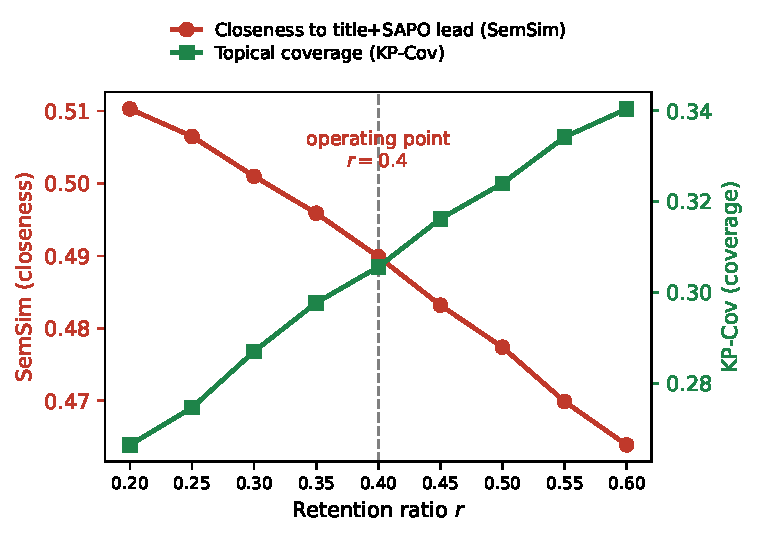
\includegraphics[width=0.92\columnwidth]{figures/retention_balance.pdf}
\caption{Đánh đổi theo tỉ lệ giữ câu $r$: độ gần lõi tiêu đề+sapo (SemSim, trục trái) giảm,
còn độ phủ chủ đề (KP-Cov, trục phải) tăng. Chúng tôi chọn $r{=}0{,}4$ làm điểm vận hành.}
\label{fig:retention}
\end{figure}

\subsection{Đánh giá trích xuất keyphrase (Tầng 2)}
Bảng~\ref{tab:keyphrase} cho thấy KeyBERT của StatLM dẫn đầu mọi độ đo. Khác biệt
giữa hai phiên bản KeyBERT (F1@10: 30,10 so với 25,51, cải thiện khoảng 18\%)
khẳng định vai trò của \emph{embedding bất đối xứng} trong việc thu hẹp khoảng
cách giữa keyphrase ngắn và tài liệu dài. WordAttractionRank dẫn đầu nhóm đồ thị
(F1@10 = 25,21) nhưng vẫn kém KeyBERT do mới dừng ở embedding mức từ và thiếu cơ
chế giảm trùng lặp như MMR.

\begin{table}[!t]
\renewcommand{\arraystretch}{1.2}
\caption{Kết quả đánh giá các phương pháp trích xuất keyphrase trên VietnamNet (đơn vị: \%)}
\label{tab:keyphrase}
\centering
\scriptsize
\setlength{\tabcolsep}{4pt}
\begin{tabular}{@{}lcccccc@{}}
\toprule
\textbf{Phương pháp} & \textbf{P@5} & \textbf{R@5} & \textbf{F1@5} & \textbf{P@10} & \textbf{R@10} & \textbf{F1@10} \\
\midrule
RAKE                       & 17,32 & 10,84 & 13,33 & 11,50 & 13,70 & 12,50 \\
YAKE                       & 20,15 & 12,67 & 15,56 & 14,45 & 17,50 & 15,83 \\
TextRank (từ khóa)         & 19,23 & 12,31 & 15,01 & 13,21 & 16,53 & 14,68 \\
TopicRank                  & 25,02 & 16,45 & 19,85 & 19,34 & 24,52 & 21,62 \\
Multipartite               & 26,83 & 17,67 & 21,31 & 20,47 & 26,26 & 23,01 \\
WordAttractionRank         & 28,49 & 17,43 & 21,63 & 23,16 & 27,66 & 25,21 \\
KeyBERT + emb. đối xứng     & 28,56 & 17,41 & 21,63 & 23,48 & 27,93 & 25,51 \\
\textbf{KeyBERT (StatLM)}  & \textbf{32,21} & \textbf{21,64} & \textbf{25,89} & \textbf{26,64} & \textbf{34,58} & \textbf{30,10} \\
\bottomrule
\end{tabular}
\end{table}

\subsection{Đánh giá không gian nhãn và phân loại (Tầng 3)}
Việc đánh giá không gian nhãn đòi hỏi cách tiếp cận hỗn hợp định lượng -- định
tính. Để bảo đảm tính khách quan khi phân loại thủ công 72 nhãn (26 của StatLM,
46 của X-MLClass-Gemini) vào năm nhóm, năm người đánh giá độc lập theo bộ hướng dẫn chuẩn
hóa. Độ nhất quán đo bằng Fleiss' $\kappa$ đạt $0{,}806$ (tỉ lệ đồng thuận thực
tế $\bar P\approx 0{,}866$, kỳ vọng ngẫu nhiên $\bar P_e\approx 0{,}307$), tương
ứng mức \emph{almost perfect} theo Landis \& Koch~\cite{landis1977}, xác nhận bộ
tiêu chí đủ tin cậy.

Bảng~\ref{tab:labelspace} so sánh cấu trúc không gian nhãn của hai hệ thống.
X-MLClass-Gemini làm việc trực tiếp trên chunk văn bản thô 50 token chứa nhiều tên riêng (``Hà
Nội'', ``VinFast'') và cụm meta báo chí (``Tin nóng 24h''); LLM không phân biệt
được chủ đề với thực thể/meta, dẫn đến 39,1\% nhãn nhiễu, đồng thời sinh 8 nhãn
đuôi dài nhưng vẫn bỏ trống 5 chuyên mục hẹp. Ngược lại, StatLM chủ động lọc
nhiễu từ hai tầng đầu: TextRank giữ câu trọng tâm, KeyBERT với lọc từ loại loại
bỏ thực thể/meta ngay khi trích keyphrase, khiến Gemini chỉ nhận 5 keyphrase sạch
và buộc phải khái quát hóa. Kết quả: không sinh Entity/Long-tail, tỉ lệ nhiễu chỉ
3,8\% và phủ 19/20 chuyên mục (gộp hợp lý các chuyên mục hẹp, ví dụ ``Bảo vệ
người tiêu dùng'' + ``Thị trường -- tiêu dùng'' $\rightarrow$ ``Tiêu dùng \& Thị
trường'').

\begin{table}[!t]
\renewcommand{\arraystretch}{1.2}
\caption{Cấu trúc và chất lượng không gian nhãn của X-MLClass-Gemini và StatLM}
\label{tab:labelspace}
\centering
\footnotesize
\begin{tabular}{@{}lcccc@{}}
\toprule
\multirow{2}{*}{\textbf{Nhóm nhãn}} & \multicolumn{2}{c}{\textbf{X-MLClass-Gemini}} & \multicolumn{2}{c}{\textbf{StatLM}} \\
\cmidrule(lr){2-3}\cmidrule(lr){4-5}
 & \textbf{SL} & \textbf{Tỉ lệ} & \textbf{SL} & \textbf{Tỉ lệ} \\
\midrule
Coarse      & 15 & 32,6\% & \textbf{20} & \textbf{76,9\%} \\
Long-tail   &  8 & 17,4\% &  0 &  0,0\% \\
Entity      &  6 & 13,0\% &  0 &  0,0\% \\
Meta/Noise  & 12 & 26,1\% &  1 &  3,8\% \\
Cross-topic &  5 & 10,9\% &  5 & 19,2\% \\
\midrule
\textbf{Tổng} & \textbf{46} & \textbf{100\%} & \textbf{26} & \textbf{100\%} \\
\midrule
Tỉ lệ nhiễu              & \multicolumn{2}{c}{39,1\%} & \multicolumn{2}{c}{\textbf{3,8\%}} \\
Chuyên mục phủ (Coarse)  & \multicolumn{2}{c}{15/20 (75\%)} & \multicolumn{2}{c}{\textbf{19/20 (95\%)}} \\
\bottomrule
\end{tabular}
\end{table}

Về khả năng gán nhãn đầu cuối, StatLM đạt $P@1=0{,}71$ và $P@3=0{,}84$, vượt xa
X-MLClass-Gemini ($P@1=0{,}49$, $P@3=0{,}63$). Nhờ 19/20 chuyên mục gốc đều có ít nhất một
nhãn Coarse tương ứng, hầu hết các bài đều có cơ hội được xếp hạng đúng ngay vị
trí 1; trong khi đó, 18 nhãn nhiễu (Entity + Meta/Noise) của X-MLClass-Gemini -- vốn không
phản ánh chủ đề -- thường chiếm mất rank 2--3 trên các bài giàu thực thể hoặc định
dạng báo chí, đẩy nhãn đúng xuống dưới.

\subsection{Đánh giá hiệu năng}
StatLM cũng nhanh hơn và rẻ hơn đáng kể. Nó giảm thời gian xử lý trung bình từ
$\sim$40 xuống $\sim$10 giây mỗi bài, giảm lượng token gửi đến LLM từ $\sim$900
xuống $\sim$30 mỗi bài (ít hơn khoảng 30 lần), và chỉ thực hiện 1 lần gọi API mỗi
bài thay vì $\sim$8 lần. Khác biệt đến từ việc StatLM chỉ gửi 5 keyphrase
($\sim$30 token) cho LLM, trong khi X-MLClass-Gemini gửi toàn bộ nội dung thô ($\sim$900
token/bài) và còn nhiều lần gọi API cho các bước phân cụm và xác minh trùng lặp.

\subsection{Phân tích ablation và thảo luận}
Bảng~\ref{tab:ablation} lượng hóa đóng góp của từng tầng (các giá trị có dấu
$\approx$ được ngoại suy theo xu hướng). Thay TextRank gốc bằng phiên bản embedding
giúp tỉ lệ coarse tăng 8--10\% và giảm nhiễu tương ứng. Bỏ Tầng~2 (gửi thẳng tóm
tắt cho LLM) khiến tỉ lệ coarse giảm mạnh từ 76,9\% xuống $\approx$55\% -- cho
thấy keyphrase là cầu nối then chốt giữa tóm tắt và LLM. Thay Tầng~2 bằng embedding
đối xứng làm F1@10 giảm khoảng 15\% và kéo nhiễu nhãn tăng gần gấp đôi. Những quan
sát này khẳng định thiết kế ``làm sạch trước, khái quát sau'' là hợp lý và từng
thành phần đều khó thay thế.

\begin{table}[!t]
\renewcommand{\arraystretch}{1.25}
\caption{Ảnh hưởng của từng tầng đến chất lượng không gian nhãn cuối cùng
(T1: ROUGE-1 F1; T2: F1@10; T3: Coarse / Nhiễu / Số chuyên mục được phủ).}
\label{tab:ablation}
\centering
\footnotesize
\begin{tabularx}{\columnwidth}{@{}Xcc>{\raggedright\arraybackslash}X@{}}
\toprule
\textbf{Biến thể} & \textbf{T1} & \textbf{T2} & \textbf{T3 (Coarse/Nhiễu/Phủ)} \\
\midrule
StatLM đầy đủ          & 0,403 & 30,10 & 76,9\% / 3,8\% / 19/20 \\
T1 $\to$ TextRank gốc  & 0,341 & $\approx$28,5 & $\approx$68\% / $\approx$10\% / 17/20 \\
Bỏ T1                  & --    & $\approx$27,0 & $\approx$65\% / $\approx$15\% / 16/20 \\
T2 $\to$ đối xứng       & 0,403 & 25,51 & $\approx$70\% / $\approx$8\% / 17/20 \\
Bỏ T2                  & 0,403 & --    & $\approx$55\% / $\approx$20\% / 14/20 \\
\bottomrule
\end{tabularx}
\end{table}

Bức tranh tổng thể làm nổi bật triết lý \emph{Statistical Encoder -- Language
Model Decoder}. X-MLClass-Gemini dù kế thừa sức mạnh của pipeline gốc vẫn bộc lộ điểm yếu khi
gặp dữ liệu báo chí thực tế: LLM bị phân tán bởi thực thể và cụm định dạng, tạo
không gian nhãn nhiễu và tốn kém. StatLM giải quyết một cách hệ thống bằng cách
chủ động lọc nhiễu trước khi dữ liệu đến LLM, cho ra không gian nhãn gọn, sạch,
tập trung vào nhãn thô (Coarse), đồng thời giảm mạnh chi phí token và thời gian.
Nói cách khác, để có một bộ nhãn thô hữu ích, một chiến lược ``làm sạch trước,
khái quát sau'' đơn giản và tiết kiệm như StatLM là đủ dùng, không cần đến một
pipeline phức tạp và đắt đỏ. Kết quả ablation (Bảng~\ref{tab:ablation}) còn cho
thấy hai tầng encoder bổ trợ chứ không thay thế lẫn nhau: Tầng~1 nâng chất lượng
đầu vào của Tầng~2, còn embedding bất đối xứng ở Tầng~2 là điều kiện cần để LLM
nhận được keyphrase đủ sạch -- cả hai cùng quyết định độ tinh gọn của không gian
nhãn cuối cùng.



% ============================================================
\section{Kết luận}
% ============================================================
Bài báo đề xuất \textbf{StatLM}, một pipeline encoder--decoder cho bài toán phân
loại văn bản đa nhãn zero-shot trong môi trường thế giới mở cho tiếng Việt. Bằng
cách giao việc giảm nhiễu và cô đặc thông tin cho encoder thống kê (TextRank trên
sentence embedding, KeyBERT với embedding bất đối xứng) và chỉ huy động LLM một lần ở
decoder, StatLM cân bằng chất lượng, chi phí và tốc độ: so với baseline X-MLClass-Gemini dùng
LLM toàn phần, nó nâng tỉ lệ nhãn thô lên 76,9\%, hạ nhiễu xuống 3,8\%, phủ 19/20
chuyên mục, và giảm token cùng thời gian khoảng $30\times$ và $4\times$.

\textbf{Hạn chế.} Chất lượng phụ thuộc dây chuyền vào hai tầng encoder; chi phí xây
đồ thị tăng $O(n^2)$ với văn bản rất dài; đầu ra LLM còn dao động nhẹ giữa các lần
chạy; và tham chiếu keyphrase là LLM-proxy chứ chưa phải ground-truth do người gán.
Chuỗi xử lý cũng là vòng hở: một chủ đề phụ chỉ nằm trong vài câu có độ trung tâm
thấp có thể bị bỏ mà không được khôi phục---một rủi ro \emph{được cơ chế dự đoán}
dưới benchmark một nhãn vàng ($|L_i|=1$), mà để định lượng cần một tập con đa nhãn do
người gán.

\textbf{Hướng phát triển.} Tích hợp thông tin vị trí câu và cấu trúc văn bản vào đồ
thị; mở rộng sang các miền khác và xây dựng bộ dữ liệu keyphrase tiếng Việt gán nhãn
thủ công; và bổ sung cơ chế dự phòng dựa trên độ tin cậy, đưa lại toàn văn vào khâu
trích keyphrase khi độ phủ bản tóm tắt hoặc độ tin cậy gán nhãn thấp, khép một phần
vòng lặp hiện hở.



% ============================================================
\section*{Lời cảm ơn}
Tác giả trân trọng cảm ơn Trường Đại học Công nghệ, Đại học Quốc gia Hà Nội đã hỗ
trợ và tạo điều kiện cho nghiên cứu.



% ============================================================
% Tài liệu tham khảo: dùng BibTeX với style IEEEtran
% ============================================================
\bibliographystyle{IEEEtran}
\bibliography{references}

\end{document}
